\chapter{Implementation}
\paragraph{} Stereoscopy is a technique used for recording and representing stereoscopic (3D) images. It can create an illusion of depth using two pictures taken at slightly different positions.
\paragraph{} Stereoscopic picture can be taken with a pair of cameras similarly to our own eyes. The most important restrictions in taking a pair of stereoscopic pictures are the following:
\begin{itemize}
	\item cameras should be horizontally aligned (see Figure 1), and
	\item the pictures should be taken at the same instant.
\end{itemize}

\begin{figure}[!h]
	\begin{subfigure}[b]{0.4\textwidth}
		\centering
		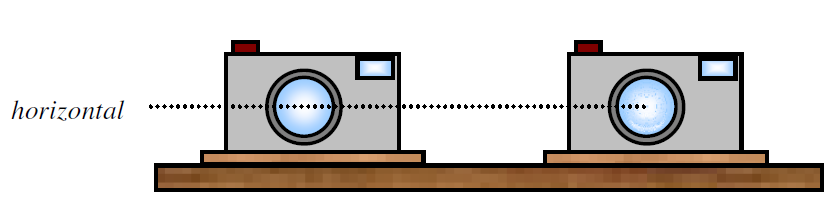
\includegraphics[width=1.3\textwidth,scale=2]{project/images/a.png}
		\caption{\textsc{Horizantal Setup}}
		\label{fig:3}
	\end{subfigure}
	\hspace{2cm}
	\begin{subfigure}[b]{0.4\textwidth}
		\centering
		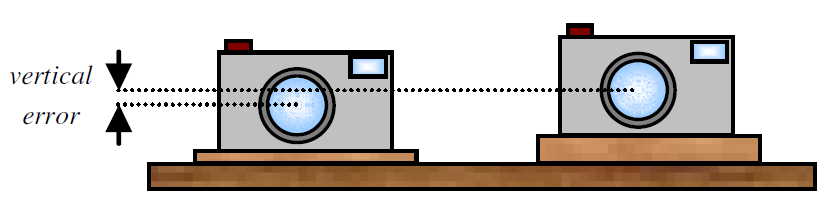
\includegraphics[width=1.3\textwidth]{project/images/b.png}
		\caption{\textsc{Vertical Setup}}
		\label{fig:4}
	\end{subfigure}\\
	\hspace{3cm}
\begin{subfigure}[b]{0.4\textwidth}
	\vspace{1cm}
	
	\centering
	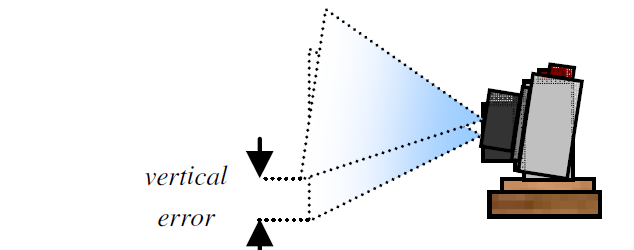
\includegraphics[width=1.3\textwidth]{project/images/c.png}
	\caption{\textsc{Angle Setup}}
	\label{fig:5}
\end{subfigure}
	\caption{\textsc{Stereo Camera Setup}}
\end{figure}
\paragraph{} Stereoscopic pictures allow us to calculate the distance between the camera(s) and the chosen object within the picture. Let the right picture be taken in location SR and the left picture in location SL. B represents the distance between the cameras and is camera’s horizontal angle of view. Object’s position (distance D) can be calculated by doing some geometrical derivations.
We can express distance B as a sum of distances $ B_{1} $ and $ B_{2} $:
\begin{equation}
B=B_{1}+B_{2}= D\tan\varphi_{1}+D\tan\varphi_{2}
\end{equation}
\paragraph{} if optical axes of the cameras are parallel, where $\varphi_{1}$ and $\varphi_{2}$ are angles between optical axis of camera lens and the
chosen object.
Distance D is as follows:
\begin{equation}
D=\frac{B}{\tan\varphi_{1}+\tan\varphi_{2}}
\end{equation}
\begin{figure}[H]
	\centering
	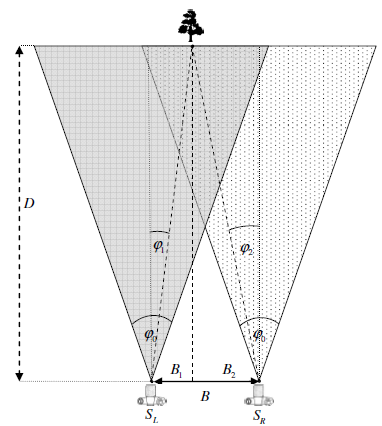
\includegraphics[height= 12cm, width=10cm]{project/images/d.png}
	\caption{\textsc{Object captured by Stereo Setup}}
\end{figure}
This figure shows the setup installed to capture Image of a \emph{tree}, the two cameras used($S_{L}$ and $S_{R}$) are similar in aspect of their \textbf{Field of View}, \textbf{Focal length}.
\newpage
\begin{figure}[h]
	\begin{subfigure}[b]{0.4\textwidth}
		\centering
		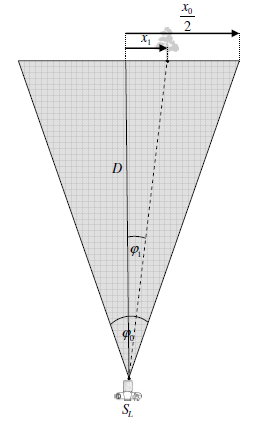
\includegraphics[width=1.3\textwidth,scale=2]{project/images/l.png}
		\caption{\textsc{Object through Left Camera}}
		\label{fig:3}
	\end{subfigure}
	\hspace{2cm}
	\begin{subfigure}[b]{0.4\textwidth}
		\centering
		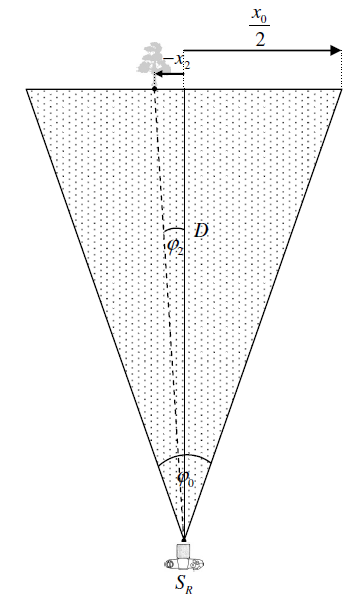
\includegraphics[width=1.3\textwidth]{project/images/r.png}
		\caption{\textsc{Object through Right Camera}}
		\label{fig:4}
	\end{subfigure}\\
	\caption{\textsc{Individual camera working}}
\end{figure}
The two separate images, give rise to two different equations as follows:
\begin{equation}
\frac{x_{1}}{\frac{x_{0}}{2}}=\frac{\tan\varphi_{1}}{\tan\frac{\varphi_{0}}{2}}
\end{equation}
\begin{equation}
\frac{-x_{2}}{\frac{x_{0}}{2}}=\frac{\tan\varphi_{2}}{\tan\frac{\varphi_{0}}{2}}
\end{equation}
Putting the deduced values of $\varphi_{1}$ and $\varphi_{2}$ in the principle equation gives an resultant form of:
\begin{equation}
D=\frac{Bx_{0}}{2\tan(\frac{\varphi_{0}}{2})(x_{1}+x_{2})}
\end{equation}
\textbf{Note:} Here $(x_{1}+x_{2})$ is represented in the form of $(x_{L}-x_{D})$ for ease of understanding.
\newpage
Therefore, if the distance between the cameras (B), number of horizontal pixels $(x_{0})$, the viewing angle of the camera$(\varphi_{0})$ and the horizontal difference between the same object on both pictures $(x_{L}-x_{D})$ are known, then the distance to the object $(D)$ can be calculated as given in  final expression.
The accuracy of the calculated position (distance D) depends on several variables. Location of the object in the right picture can be found within accuracy of one pixel. Each pixel corresponds to the following angle of view:\\
\begin{equation}
\delta=\frac{\varphi_{0}}{x_{0}}
\end{equation}
\\one pixel angle of view $\delta\varphi$ results in distance error $\delta D$. In image we find:
\begin{equation}
\frac{\tan\varphi}{\tan(\varphi-\delta\varphi)}=\frac{\delta D+D}{D}
\end{equation}
Using basic trigonometry identities, the distance error can be expressed as follows:\\
\begin{equation}
\delta D= \frac{D^{2}}{B}\tan(\delta\varphi)
\end{equation}
\begin{figure}[H]
	\centering
	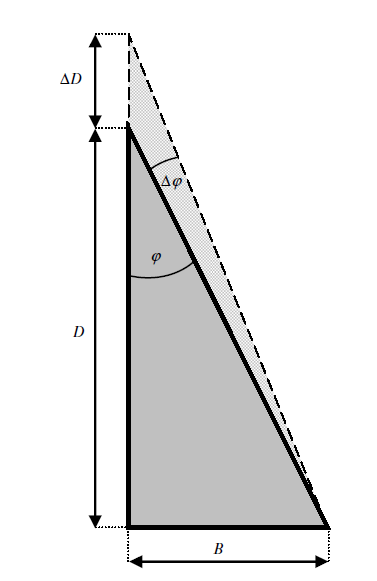
\includegraphics[height= 12cm, width=10cm]{project/images/z.png}
	\caption{\textsc{Distance Error caused by $1$ pixel}}
\end{figure}